\documentclass[12pt]{beamer}

\usecolortheme[dark,accent=yellow]{solarized}
\beamertemplatetransparentcovered
\setbeamertemplate{navigation symbols}{} % remove navigation symbols
% \setbeamertemplate{footline}[page number]
\setbeamertemplate{footline}{
  \hfill%
  \usebeamercolor[fg]{page number in head/foot}%
  \usebeamerfont{page number in head/foot}%
  \setbeamertemplate{page number in head/foot}[framenumber]%
  \usebeamertemplate*{page number in head/foot}\kern1em\vskip2pt%
}
\setbeamerfont{page number in head/foot}{size=\small}

\usepackage[german]{babel}
\usepackage{times}
\usepackage{esvect}\renewcommand{\vec}[1]{\vv{#1}}
\usepackage{setspace}\setstretch{1.5}
\usepackage{tikz}
\usepackage{pgfplots}\pgfplotsset{compat=1.17}
\usepackage{siunitx}

%%%%%%%%%%%%%%%%%%%%%%%%%%%%%%%%%%%%%%%%%%%%%%%%%%

\usetikzlibrary{calc,decorations.markings}

% default arrow style
\tikzset{>=latex}

% arrows on the field lines
\tikzstyle directed=[postaction={decorate,decoration={markings,
  mark=at position .2 with {\arrowreversed[scale=1.5]{>}},
  mark=at position .8 with {\arrowreversed[scale=1.5]{>}}}}]

% field lines
\tikzstyle fLines=[thick,directed]

\newcommand{\magnet}[3]{%
    \def\lmag{#1}  % length of magnet
    \def\wmag{#2}  % thickness of magnet
    \def\nc{#3}    % no. of lines = 2*\nc+1
    \begin{scope}
      \coordinate (A) at (-\lmag/2,\wmag/2);
      \coordinate (B) at (\lmag/2,-\wmag/2);
      \draw[fill, color=green](A) rectangle ++(\lmag/2,-\wmag) node[black,midway]{S};
      \draw[fill, color=red](0,-\wmag/2) rectangle ++(\lmag/2,\wmag) node[black,midway]{N};
      \clip (-5,-3) rectangle (5,3);
      \foreach \r in {1,...,\nc}{
        \draw[fLines]($(A)-(0,0.5*\r*\wmag/\nc)$) arc(({270-asin(\lmag/(2*\r))}):({-90+asin(\lmag/(2*\r))}):\r);
        \draw[fLines]($(B)+(0,0.5*\r*\wmag/\nc)$) arc(({90-asin(\lmag/(2*\r))}):({-270+asin(\lmag/(2*\r))}):\r); }
      \draw[fLines] (-\lmag/2,0) -- ++(-6,0);
      \draw[fLines] (\lmag/2,0) ++(6,0)--(\lmag/2,0);
    \end{scope}
    \draw[blue,->,line width=3] (-\nc/8,2) -- ++(\nc/4,0) node[midway,above] {$\vec{m}$};
}

%%%%%%%%%%%%%%%%%%%%%%%%%%%%%%%%%%%%%%%%%%%%%%%%%%

\newcommand{\Exp}{\text{Exp}}
\newcommand{\SM}{\text{SM}}

% BNL-E821
\newcommand{\amuBNL}{11659209.1} % 
\newcommand{\numamuBNL}{\num{\amuBNL}}
\newcommand{\DamuBNL}{6.3}

% FNAL 2021
\newcommand{\amuFNAL}{11659204.0}
\newcommand{\DamuFNAL}{5.4}
\newcommand{\numamuFNAL}{\num{\amuFNAL}}

% experimental, combined
\newcommand{\amuExp}{11659206.1}
\newcommand{\numamuExp}{\num{\amuExp}}
\newcommand{\DamuExp}{4.1} % uncertainty

% SM
\newcommand{\amuSM}{11659181.0}
\newcommand{\numamuSM}{\num{\amuSM}}
\newcommand{\DamuSM}{4.3}

\definecolor{blue}{rgb}{0,0.7,1.0}
\definecolor{green}{rgb}{0,1.0,0.5}

%%%%%%%%%%%%%%%%%%%%%%%%%%%%%%%%%%%%%%%%%%%%%%%%%%

\title{The magic is always in the details}
\subtitle{The search for new physics with the muon}

\author[Voigt]{Alexander Voigt}
\institute[HS Flensburg]{Hochschule Flensburg}
\date{Planetarium Talks 2022}

\begin{document}

%%%%%%%%%%%%%%%%%%%%%%%%%%%%%%%%%%%%%%%%%%%%%%%%%%

\begin{frame}
  \titlepage
\end{frame}

%%%%%%%%%%%%%%%%%%%%%%%%%%%%%%%%%%%%%%%%%%%%%%%%%%

\begin{frame}{Table of Contents}
  \tableofcontents
\end{frame}

%%%%%%%%%%%%%%%%%%%%%%%%%%%%%%%%%%%%%%%%%%%%%%%%%%

\section{Magnetism}

\begin{frame}{\insertsection: permanent magnet}
  \begin{center}
    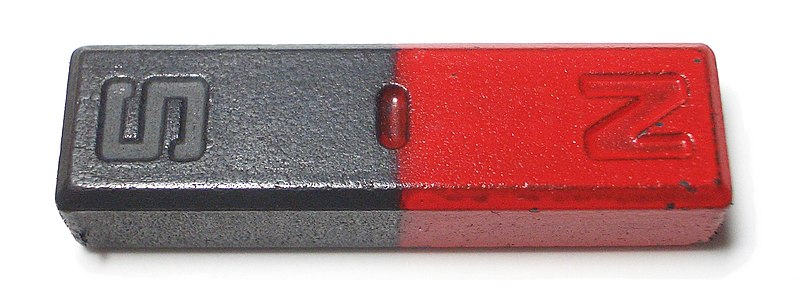
\includegraphics[width=0.9\textwidth]{img/bar_magnet_foto}

    \footnotesize [Aney, CC-SA-3.0]
  \end{center}
\end{frame}

\begin{frame}{\insertsection: magnetic moment $\vec{m}$}
  \begin{tikzpicture}
    \only<1>{\magnet{1.8}{0.5}{3}}%
    \only<2>{\magnet{1.8}{0.5}{4}}%
    \only<3>{\magnet{1.8}{0.5}{5}}%
    \only<4>{\magnet{1.8}{0.5}{6}}%
    \only<5>{\magnet{1.8}{0.5}{7}}%
    \only<6>{\magnet{1.8}{0.5}{8}}%
    \only<7>{\magnet{1.8}{0.5}{9}}%
    \only<8>{\magnet{1.8}{0.5}{10}}%
    \only<9>{\magnet{1.8}{0.5}{11}}%
  \end{tikzpicture}  
\end{frame}

% \begin{frame}{\insertsection}
%   Magnetisches Moment $\vec{m}$:
%   \begin{itemize}
%   \item Beschreibt WW eines magnetischen Dipols mit einem Magnetfeld
%   \item Betrag: "`Stärke der WW"'
%   \item Richtung: Angestrebte Ausrichtung zum Magnetfeld
%   \end{itemize}
%   Ursache des Magnetismus bei einem Permanentmagneten:
%   \begin{itemize}
%   \item Bahndrehimpuls
%   \item Spin
%   \end{itemize}
%   der Atome
% \end{frame}

\begin{frame}{\insertsection: origin}
  \begin{center}
    \begin{tikzpicture}
      \def\lmag{1.8}  % length of magnet
      \def\wmag{0.5}  % thickness of magnet
      \coordinate (A) at (-\lmag/2,\wmag/2);
      \coordinate (B) at (\lmag/2,-\wmag/2);
      \draw[fill, color=green](A) rectangle ++(\lmag/2,-\wmag) node[black,midway]{S};
      \draw[fill, color=red](0,-\wmag/2) rectangle ++(\lmag/2,\wmag) node[black,midway]{N};
    \end{tikzpicture}
  \end{center}
\end{frame}

\begin{frame}{\insertsection: origin}
  \begin{center}
    \begin{tikzpicture}
      \def\lmag{4}  % length of magnet
      \def\wmag{1}  % thickness of magnet
      \coordinate (A) at (-\lmag/2,\wmag/2);
      \coordinate (B) at (\lmag/2,-\wmag/2);
      \draw[fill, color=green](A) rectangle ++(\lmag/2,-\wmag) node[black,midway]{\large S};
      \draw[fill, color=red](0,-\wmag/2) rectangle ++(\lmag/2,\wmag) node[black,midway]{\large N};
      %
      \foreach \X in {-1.9,-1.7,...,1.9} {%
        \foreach \Y in {-0.4,-0.2,...,0.4} {%
          \draw[fill,black] (\X,\Y) circle (0.01);
        }
      }
    \end{tikzpicture}
  \end{center}
\end{frame}

\begin{frame}{\insertsection: origin}
  \begin{center}
    \begin{tikzpicture}
      \def\lmag{8}  % length of magnet
      \def\wmag{2}  % thickness of magnet
      \coordinate (A) at (-\lmag/2,\wmag/2);
      \coordinate (B) at (\lmag/2,-\wmag/2);
      \draw[fill, color=green](A) rectangle ++(\lmag/2,-\wmag) node[black,midway]{\Huge S};
      \draw[fill, color=red](0,-\wmag/2) rectangle ++(\lmag/2,\wmag) node[black,midway]{\Huge N};
      %
      \foreach \X in {-3.8,-3.4,...,3.9} {%
        \foreach \Y in {-0.8,-0.4,...,0.9} {%
          \draw[fill,black] (\X,\Y) circle (0.02);
        }
      }
    \end{tikzpicture}
  \end{center}
\end{frame}

\begin{frame}{\insertsection: origin}
  \begin{center}
    \begin{tikzpicture}
      \def\lmag{8}  % length of magnet
      \def\wmag{2}  % thickness of magnet
      \coordinate (A) at (-\lmag/2,\wmag/2);
      \coordinate (B) at (\lmag/2,-\wmag/2);
      \draw[fill, color=green](A) rectangle ++(\lmag/2,-\wmag) node[black,midway]{\Huge S};
      \draw[fill, color=red](0,-\wmag/2) rectangle ++(\lmag/2,\wmag) node[black,midway]{\Huge N};
      %
      \foreach \X in {-3.8,-3.4,...,3.9} {%
        \foreach \Y in {-0.8,-0.4,...,0.9} {%
          % \draw[fill,black] (\X,\Y) circle (0.02);
          \draw[black,->] (\X-0.1,\Y) -- ++(0.2,0);
        }
      }
    \end{tikzpicture}
  \end{center}
\end{frame}

\begin{frame}{\insertsection: origin}
  \begin{center}
    \begin{tikzpicture}
      \fill[even odd rule,inner color=blue,outer color=solarizedRebase03!100] (0,0) circle (3);
      \coordinate (n) at (0,0);
      \coordinate (e) at (2,0.5);
      \draw[fill,red] (n) circle (0.1);
      \draw[fill,green] (e) circle (0.05);
      \only<1>{%
        \node[below,black] at (n) {nucleus};
        \node[below,green] at (e) {electron};
      }%
      \only<2>{%
        \draw[very thick,red,->] ($(n)+(0,-1)$) -- ++(0,2);
        \draw[very thick,green,->] ($(e)+(0,-0.5)$) -- ++(0,1);
      }%
      \only<1-2>{%
        \draw[ultra thick,blue,->] (5,-1.5) -- node[right] {$\vec{m}$} ++(0,3);
      }%
    \end{tikzpicture}
  \end{center}
\end{frame}

%%%%%%%%%%%%%%%%%%%%%%%%%%%%%%%%%%%%%%%%%%%%%%%%%%

\section{What the world is made of}

\begin{frame}{\insertsection}
  The Standard Model of Particle Physics:
\end{frame}

%%%%%%%%%%%%%%%%%%%%%%%%%%%%%%%%%%%%%%%%%%%%%%%%%%

\section{Open questions}

\begin{frame}{\insertsection}
  \begin{itemize}
  \item Dark Matter
  \item Unification of Forces
  \item Hierarchy Problem
  \end{itemize}
\end{frame}

%%%%%%%%%%%%%%%%%%%%%%%%%%%%%%%%%%%%%%%%%%%%%%%%%%

\section{Anomalous magnetic moment}

\begin{frame}{\insertsection}
  Relative deviation of $g$ from the value 2:
  \begin{align*}
    a := \frac{g-2}{2}
  \end{align*}
\end{frame}

%%%%%%%%%%%%%%%%%%%%%%%%%%%%%%%%%%%%%%%%%%%%%%%%%%

\section{Measurement}

\begin{frame}{\insertsection}
  Exprimental measurements:
  \begin{align*}
    a^{\text{BNL}} &= (\numamuBNL \pm \DamuBNL)\times 10^{-10} && (2016)\\
    a^{\text{FNAL}} &= (\numamuFNAL \pm \DamuFNAL)\times 10^{-10} && (2021)
    \intertext{Combined:}
    a^{\Exp} &= (\numamuExp \pm \DamuExp)\times 10^{-10}
  \end{align*}
\end{frame}

%%%%%%%%%%%%%%%%%%%%%%%%%%%%%%%%%%%%%%%%%%%%%%%%%%

\section{Prediction}

\begin{frame}{\insertsection}
  Standard Model prediction:
  \begin{align*}
    a^\SM &= (\numamuSM \pm \DamuSM)\times 10^{-10}
  \end{align*}
\end{frame}

%%%%%%%%%%%%%%%%%%%%%%%%%%%%%%%%%%%%%%%%%%%%%%%%%%

\section{Comparison of measurement and prediction}

% \begin{frame}{\insertsection}
%   \begin{align*}
%     a^{\Exp} &= (\numamuExp \pm \DamuExp)\times 10^{-10} \\
%     a^\SM &= (\numamuSM \pm \DamuSM)\times 10^{-10} \\
%     \Rightarrow\qquad
%     a^{\Exp} - a^\SM &= (25.1 \pm 5.9)\times 10^{-10}
%   \end{align*}
% \end{frame}

\begin{frame}{\insertsection}
  \begin{columns}
    \column{0.7\textwidth}
    \begin{center}
      \begin{tikzpicture}
        \begin{axis}[
          width=\textwidth,
          height=0.8\textheight,
          xlabel = {$(a - a^\SM)\times 10^{10}$},
          ymajorticks = false,
          xmin = -10, xmax = 40,
          ymin = 0, ymax = 4,
          ]
          \addplot[blue,dashed,only marks,mark=*,error bars/.cd,x dir=both, x explicit] coordinates {
            (\amuBNL  - \amuSM, 3) +- (\DamuBNL , 0)
            (\amuFNAL - \amuSM, 2) +- (\DamuFNAL, 0)
            % (\amuExp  - \amuSM, 1) +- (\DamuExp , 0)
          };
          \addplot[blue,only marks,mark=*,error bars/.cd,x dir=both, x explicit] coordinates {
            (\amuExp  - \amuSM, 1) +- (\DamuExp , 0)
          };
          \draw[fill,green] (-\DamuSM, 0) rectangle (\DamuSM, 4);
          \node[above] at (\amuBNL  - \amuSM, 3) {BNL};
          \node[above] at (\amuFNAL - \amuSM, 2) {FNAL};
          \node[above] at (\amuExp  - \amuSM, 1) {Experiment};
          \node[black,rotate=90] at (0, 2) {SM prediction};
        \end{axis}
      \end{tikzpicture}
    \end{center}

    \column{0.29\textwidth}
    $a^{\Exp} - a^\SM = (25.1 \pm 5.9)\times 10^{-10}$

    \bigskip

    Deviation $\approx 4.2\sigma$

    \bigskip

    % using SpecialFunctions
    % DF(n) = erf(n/sqrt(2))
    % (1 - DF(4.2))*100

    $P(\text{data}|\SM)\approx \num{0.0027}\%$

  \end{columns}
\end{frame}

%%%%%%%%%%%%%%%%%%%%%%%%%%%%%%%%%%%%%%%%%%%%%%%%%%

\section{How can we explain the deviation?}

\begin{frame}{\insertsection}
  Möglicher Grund für Abweichung: Es gibt noch weitere unentdeckte
  Elementarteilchen!
  \begin{itemize}
  \item zusätzliche Higgs-Teilchen?
  \item zusätzliche Quarks oder Leptonen?
  \item Supersymmetrie?
  \end{itemize}
\end{frame}

\end{document}
